% Indicate the main file. Must go at the beginning of the file.
% !TEX root = ../main.tex

%%%%%%%%%%%%%%%%%%%%%%%%%%%%%%%%%%%%%%%%%%%%%%%%%%%%%%%%%%%%%%%%%%%%%%%%%%%%%%%%
% 02_methods
%%%%%%%%%%%%%%%%%%%%%%%%%%%%%%%%%%%%%%%%%%%%%%%%%%%%%%%%%%%%%%%%%%%%%%%%%%%%%%%%

\section{Methods}
\label{methods}

\subsection{Data}%%%%%%%%%%%%%%%%%%%%%%%%%%%%%%%%%%%%%%%%%%%%%%%%%%%%%%%%%%%%%%%

The used data for this project is the SwissImage RS data from the Swiss Federal Office of Topography (swisstopo).
It is a raster dataset with a resolution of 0.1m containing four bands: RGB and NIR.
In order to cover the area of interest (AOI) 6 tiles of the dataset are needed.
Over this large AOI there are three areas labeled with the corresponding landcover categories.
This labeled data was provided by a team of researchers from the ZHAW. The three
areas are distributed over a residential area (83487m\textsuperscript{3}),
qn industrial area (132642m\textsuperscript{3}) and a rural area (82740m\textsuperscript{3}) \autoref{fig:category_areas}.
There are 10 different landcover categories in total shown in \autoref{fig:landcover_categories}.

\begin{figure}[H]
    \centering
    \captionsetup{width=0.8\linewidth}
    \includegraphics[width=\linewidth]{figures/category_areas.png}
    \caption{The three areas with the corresponding landcover categories.}
    \label{fig:category_areas}
\end{figure}

\begin{figure}[H]
    \centering
    \captionsetup{width=0.8\linewidth}
    \includegraphics[scale=0.6]{figures/area_by_category.pdf}
    \caption{Landcover categories in the labeled areas summed up by shape area}
    \label{fig:landcover_categories}
\end{figure}

\subsection{Data Processing}%%%%%%%%%%%%%%%%%%%%%%%%%%%%%%%%%%%%%%%%%%%%%%%%%%%%

In a first step the data was processed using ArcGIS Pro. The process included a few steps implemented as
a model \autoref{fig:processing_model}. The 6 tiles where mosaiced together and the area of interest 
was clipped. The landcover categories where transformed into a raster dataset and added as aditional
band as well as an extra mask band constructed for orientation purposes. To get an overview of the
available data refer to \autoref{fig:aoi_labeled}. The data was then exported as a GeoTIFF file.
In order to use the data in a neural network an additional step was necessary. Using a custom Python script,
the data was transformed into Zarr format. This format is a chunked, compressed, N-dimensional array
storage format with multi-scale support. This allows for lazy loading and therefore for a more memory
efficient data access during training.

\begin{figure}[H]
    \centering
    \captionsetup{width=0.8\linewidth}
    \includegraphics[scale=0.6]{figures/AOI_Labeled.png}
    \caption{The area of interest with the three labeled areas.}
    \label{fig:aoi_labeled}
\end{figure}

\begin{figure}
    \centering
    \captionsetup{width=0.8\linewidth}
    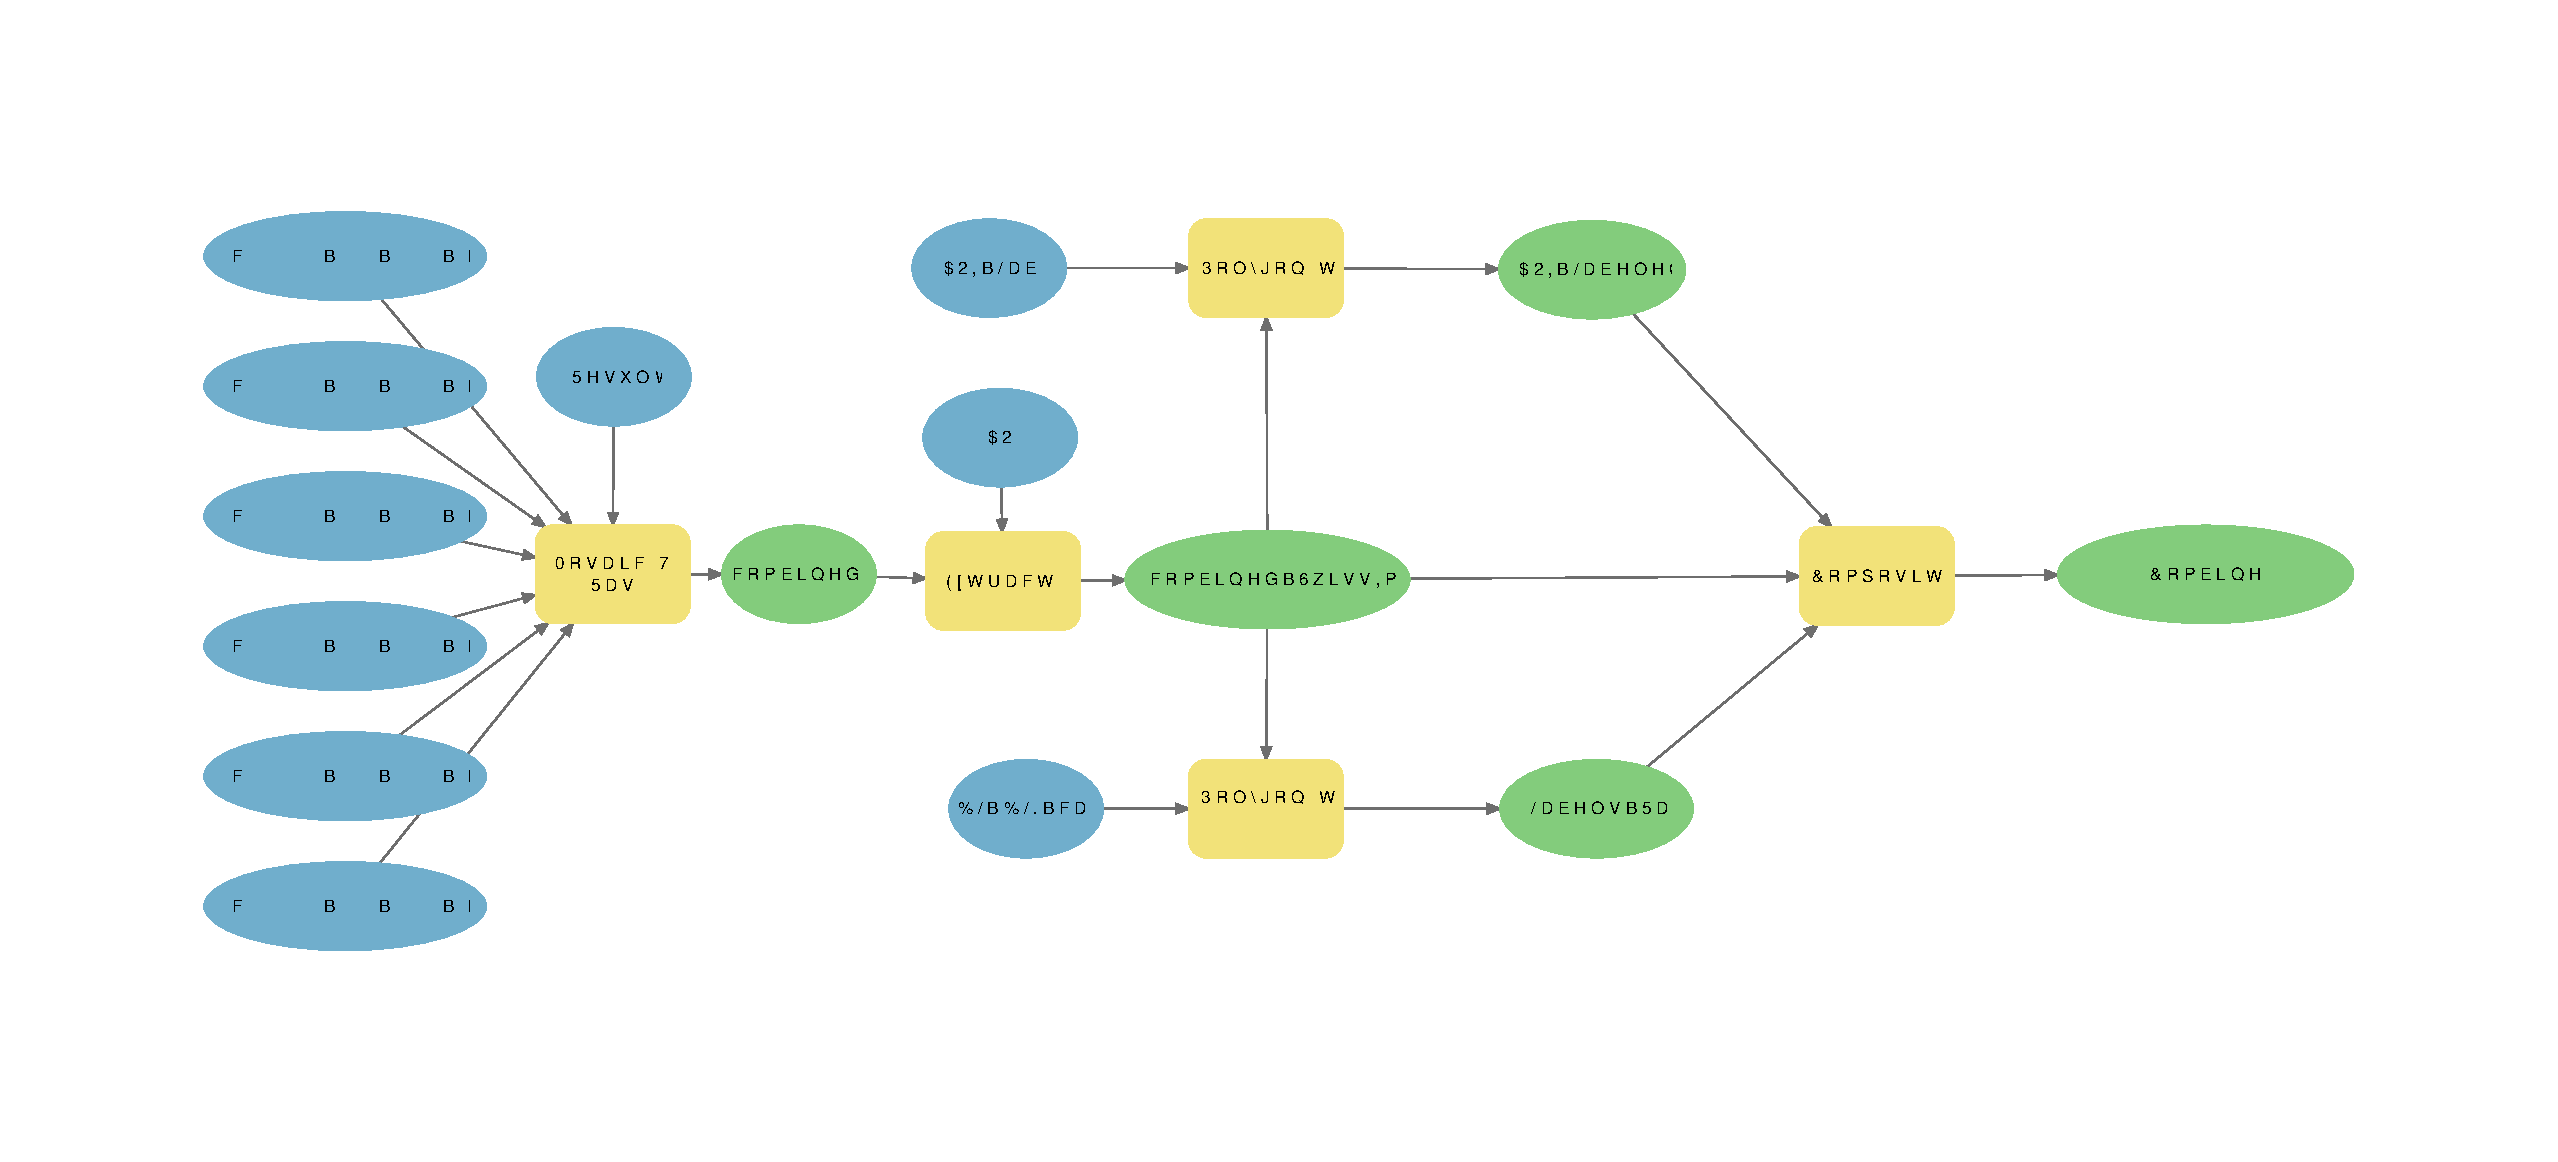
\includegraphics[width=\linewidth]{figures/Model.pdf}
    \caption{The ArcGis model used for preprocessing the data.}
    \label{fig:processing_model}
\end{figure}

\subsection{Data Loader and Augmentation}%%%%%%%%%%%%%%%%%%%%%%%%%%%%%%%%%%%%%%%%

